


\section{Relevant text detection}
\label{cp4:corpus-relevant-text}


Provided that we have a set of software tasks and pertinent artifacts associated with each task, 
the last step in our corpus creation pipeline is the detection of relevant information within 
each pertinent artifact. To that end, we rely on state-of-the-art approaches able to automatically identify relevant text for the tasks and artifacts in our corpus~\cite{nadi2020, Robillard2015, Lotufo2012, Xu2017}.


To identify techniques applicable to the creation of our corpus, we systematically reviewed related work. We searched for techniques based on their availability in existing replication packages and their readiness for use.
We also refrained from using approaches with training procedures (e.g., ~\cite{liu2020} or ~\cite{Treude2016}) because of the challenges related to correctly tuning such supervised approaches~\cite{Chaparro2017, fucci2019}. Based on these criteria, three techniques were selected for the following sources in parenthesis:


\begin{itemize}[leftmargin=\parindent, font=\normalfont\itshape]
    \item \texttt{\acs{AnsBot}} (\textit{SO Answers}) uses several features (e.g., information entropy, textual patterns, entity overlap, etc.) to determine that a sentence has useful information to a developer's technical question~\cite{Xu2017}.
    
    \item \texttt{\acs{Krec}} (\textit{API Documentation}) identifies text fragments that reflect ``potentially important text that programmers cannot afford to ignore when using the API''~\cite{Robillard2015}.
    
    \item \texttt{\acs{Hurried}} (\textit{GitHub issues}) identify the most relevant sentences in a bug report based on three factors used to assess a sentence's relevancy (i.e., sentence's prominence in the issue, topic, and its similarity to the task)~\cite{Lotufo2012}.
\end{itemize}



While our corpus also has miscellaneous Web pages, we are not aware of a technique able to identify task relevant text for it. We detail how we make use of miscellaneous sources in Section~\ref{}.


For the pertinent artifacts of our running example (Figure~\ref{fig:lock-screen-task}), 
Tables~\ref{tbl:git-example-ansbot} to~\ref{tbl:git-example-hurried}
illustrate sentences automatically detected by \acs{AnsBot}, \acs{Krec}, and \acs{Hurried}, respectively.
 
% The techniques precision range from 71\% (\texttt{HurriedBug}) to 90\% (\texttt{APIRef}) and thus, we observe some unrelated sentences,
% such as a sentence expressing gratitude in Table~\ref{tbl:git-example-ansbot}.



\begin{table}[H]
\centering    
\begin{scriptsize}
\begin{threeparttable}
\rowcolors{2}{}{lightgray}
\begin{tabular}{ll}

\hline
\multicolumn{2}{c}{\textit{How to add MediaPlayer controls on lock screen?}} \\
\hline
\hline

1 & \parbox[l][.8cm][c]{10.5cm}{I had the same problem, and well, the solution was simple, do not use any widget, simply use the RemoteControlClientCompat class.} \\
2 & \parbox[l][.8cm][c]{10.5cm}{Here is my lockScreenControls() method code, which I call whenever I want to show this type of control (when plays a song).} \\
3 & \parbox[l][.5cm][c]{10.5cm}{Thank @ianhlake for the good 2 video} \\

\hline


\end{tabular}
\end{threeparttable}
\end{scriptsize}
\caption{Pertinent sentences automatically detected by \acs{AnsBot}}
\label{tbl:git-example-ansbot}
\end{table}

\begin{table}[H]
\centering    
\begin{scriptsize}
\begin{threeparttable}
\rowcolors{2}{}{lightgray}
\begin{tabular}{ll}
    
\hline
\multicolumn{2}{c}{\textit{Lock task mode - Android Developers}} \\
\hline
\hline

1 & \parbox[l][.8cm][c]{10.5cm}{You might use lock task mode if you're developing a kiosk application or a launcher to present a collection of apps.} \\
2 & \parbox[l][.8cm][c]{10.5cm}{To check if the current app is running in lock task mode, use the methods on ActivityManager as shown in the following example:} \\
3 & \parbox[l][.8cm][c]{10.5cm}{You can call KeyguardManager methods to find out if the device is locked and use an Activity lifecycle callback (such as onResume() that's called after unlocking) to start lock task mode.} \\
\hline

\end{tabular}
\end{threeparttable}
\end{scriptsize}
\caption{Pertinent sentences automatically detected by \acs{Krec}}
\label{tbl:git-example-krec}
\end{table}

\begin{table}[H]
\centering    
\begin{scriptsize}
\begin{threeparttable}
\rowcolors{2}{}{lightgray}
\begin{tabular}{ll}

\hline
\multicolumn{2}{c}{\textit{How to add MediaPlayer controls on lock screen?}} \\
\hline
\hline

1 & \parbox[l][.8cm][c]{10.5cm}{I had the same problem, and well, the solution was simple, do not use any widget, simply use the RemoteControlClientCompat class.} \\
2 & \parbox[l][.8cm][c]{10.5cm}{Here is my lockScreenControls() method code, which I call whenever I want to show this type of control (when plays a song).} \\
3 & \parbox[l][.5cm][c]{10.5cm}{Thank @ianhlake for the good 2 video} \\

\hline


\end{tabular}
\end{threeparttable}
\end{scriptsize}
\caption{Pertinent sentences automatically detected by \acs{Hurried}}
\label{tbl:git-example-hurried}
\end{table}







\subsection{Ratio of Task-relevant Sentences}
\label{cp4:evaluation}


To construct our corpus, we apply a set of techniques 
to artifacts outside the ones where the techniques were originally proposed and evaluated~\cite{nadi2020, Robillard2015, Lotufo2012, Xu2017}.
For instance, \acs{AnsBot}'s design was based on general Java programming questions~\cite{Xu2017} while the tasks in our corpus comprise Android development and originate both from GitHub and from Stack Overflow. Because of such differences, we ask:


\begin{enumerate}[label={},leftmargin=0.7cm]
\item \textit{What is the ratio of sentences relevant to the tasks and artifacts in our corpus?} 

\end{enumerate}


% Generalizability is a common threat emphasized in each of the techniques original studies~\cite{Xu2017, Lotufo2012, Robillard2015} and thus, there is a risk that the techniques do no apply to 
% the tasks and artifacts in our corpus.


Answering this question will assist in defining \textit{thresholds} or the \textit{ratio}
of the text in each artifact that has information useful to a particular task.
In turn, this information will allow us to use the \acs{DS-android} corpus for evaluating techniques that automatically identify task-relevant text across heterogeneous sources (Chapter~\ref{ch:identifying}).



We rely on three reference answers produced by 
experienced software developers to define \textit{golden relevant sentences} 
for a sample of 10 tasks and associated artifacts in our corpus. 
We then use the golden data to compute the ratio of relevant text in our corpus.




\subsubsection{Golden Data}


Creating golden data for the entirety of the \acs{DS-android} corpus is infeasible
since it would require asking human evaluators to inspect thousands of artifacts and more than 260,000 sentences.
Due to this reason, we restrict this step of our corpus creation pipeline to a random subset of 10 tasks in our corpus (i.e., 5 GitHub tasks and 5 Stack Overflow tasks). 
From now on, we refer to this subset as the \textbf{\acs{DS-android-small}} corpus.


For each one of the tasks in the \acs{DS-android-small} corpus, we also randomly selected 
one artifact per source type with and associated technique, i.e., one API document, a Github issue discussion, one Stack Overflow answer as well as two randomly selected blog or Web tutorials for a maximum of 5 artifacts per tasks.

%  TODO: update this once I review the web tutorials/blogs
% Overall, this corpus has 2,375 sentences with an average of 64 sentences per artifact---
% a size comparable to the \acs{DS-synthetic} corpus~\cite{marques2020}.
% ($\mypm$ 72)


We asked human evaluators to read the content of these artifacts and 
to mark sentences that they deemed useful and that provide information that assisted task completion---instructions similar to the ones used for the creation of the 
data in the \acs{DS-synthetic} corpus~\cite{marques2020}.



Golden data in \acs{DS-android-small} consists of any sentence that evaluators have deemed as useful for task-completion. 
Our decision to consider any sentence marked by an annotator is based on 
how individuals used different criteria to
assess relevance~\cite{Barry1994, Barry1998, Freund2015}.
There are no guarantees that
developers will use the same properties to determine text relevant to their tasks~\cite{Freund2013, Freund2015} and the text selected by a single annotator may still be crucial for task completion~\cite{marques2020}.


Due to this reason, we use a sliding scale to compute the ratio of task-relevant text in an artifact based on the golden data, i.e., 
as when one, two or the three annotators have deemed a sentence as relevant. More details on the rationale for this decision are discussed under threats to the corpus creation (Section~\ref{cp4:threats}).




\subsubsection{Annotators}
\textcolor{white}{force ident} % this is just for the chapter outline

--- We recruited \red{n} graduate students with professional programming experience to produce \textit{golden} data for our tasks sample. \vspace{3mm}


\subsubsection{Annotation Procedures}

Our intention is that goldens reflect text that a experienced developer would deem as useful for task completion and that they would share with someone eager to make their \textit{first contribution} in an open-source project.


To produce such data, annotators had  at their disposal a set of randomly assigned task descriptions and links to artifacts pertinent to the respective task. We asked annotators to write a short plan (250 words max~\cite{Rastkar2010}) with instructions that a newcomer could follow to successfully complete the task. 
The purpose of the plan was to ensure that annotators built enough context about the task.
While perusing artifacts, annotators also had to manually highlight sentences that they deemed useful and that provided information that assisted task completion. 


The annotation process was facilitated by an in-house tool, in the form of a Web browser plugin shown in Figure~\ref{fig:corpus-annotation-tool}. In the figure, the top-right corner panel shows the browser extension. Annotators could start an annotation session and click the highlight buttom.
This would instrument the HTML of a page and identify each sentence in a paragraph. The tool allowed annotators to hove over individual sentences and select them as relevant (text in orange) by clicking on the hovered text. For example, the figure depicts that an annotator selected  the sentence
``\textit{Call {\small \texttt{ActivityOptions.setLockTaskEnabled()}} ... when starting the activity}'' as relevant for the lock mode task.


\begin{figure}
    \centering
    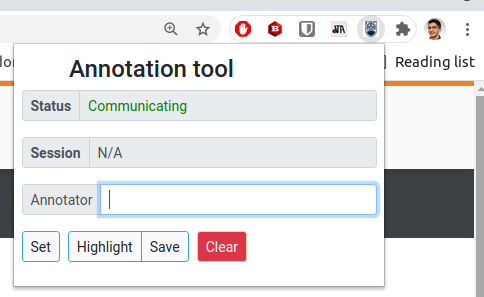
\includegraphics[width=\textwidth]{cp4/annotation-tool}
    \caption{Annotation tool and relevant sentences marked by an annotator}
    \label{fig:corpus-annotation-tool}
\end{figure}



\subsection{Evaluation Metrics}

For each task in \acs{DS-android-small}, we have a set of artifacts with task-relevant sentences identified by experienced developers. We  
compute a technique's accuracy using standard \textit{precision} and \textit{recall} metrics~\cite{Manning2009IR} by comparing the relevant text automatically identified by a technique
against the golden relevant text.



To ease interpreting evaluation metrics, Table~\ref{tbl:type-I-II-errors} show all possible evaluation outcomes. The \textit{relevant} and \textit{not-relevant} columns represent the text 
marked (or not) by the annotators. Rows represent the text automatically identified by a technique.




\begin{table}[H]
\centering    
\begin{scriptsize}
\begin{threeparttable}
\begin{tabular}{l|l|l}

\hline

\textbf{}
& \textbf{Relevant}    
& \textbf{Not-relevant} \\

\hline
\hline

\textbf{Identified as relevant} & true positive ($TP$) & false positive ($FP$) \\
\hline
\textbf{Identified as Not-relevant} & false negative ($FN$) & true negative ($TN$) \\
\hline

\end{tabular}
\end{threeparttable}
\end{scriptsize}
\caption{Result outcomes}
\label{tbl:type-I-II-errors}
\end{table}

    



For a given task $t$ and artifact $a$, precision is the ratio between the sentences identified that are marked as relevant and the total number of sentences identified, as shown in Equation~\ref{eq:cp4:precision}.


\begin{equation}
\label{eq:cp4:precision}    
    Precision(t, a) = \frac{TP}{TP + FP}
\end{equation}


Recall represents how many of all marked sentences are identified by a technique (Equation~\ref{eq:cp4:recall}).



\begin{equation}
\label{eq:cp4:recall}        
    Recall(t, a) = \frac{TP}{TP + FN}
\end{equation}

\vspace{3mm}




\subsection{Results}
\textcolor{white}{force ident} % this is just for the chapter outline


--- Discuss results. ~\red{think which summary tables should I have in the thesis body and which I can move to Appendices} \vspace{3mm}



--- Precision~\ref{tbl:ds-small-results-precision}  \vspace{3mm}


--- Recall~\ref{tbl:ds-small-results-recall} \vspace{3mm}

--- Likely explanation for the results obtained.

% When interpreting results, we favor precision instead of recall.
% A false positives may contribute to a developer abandoning reading of an artifact that would otherwise provide crucial information for her task~\cite{Rastkar2010}.




\begin{table}[H]
\centering    
\begin{scriptsize}
\begin{threeparttable}
\begin{tabular}{lcccccc}

\hline


\multirow{2.5}{*}{Technique}
& \multicolumn{2}{c}{\textit{$Precision_{n=3}$}}
& \multicolumn{2}{c}{\textit{$Precision_{n=2}$}}
& \multicolumn{2}{c}{\textit{$Precision_{n=1}$}}
\\ \cmidrule(l){2-3} \cmidrule(l){4-5} \cmidrule(l){6-7} 


& \textit{mean}
& \textit{std}
& \textit{mean}
& \textit{std}
& \textit{mean}
& \textit{std}
\\


\hline
\hline

\acs{AnsBot} 
& 0.5 & 0.5 % = 3
& 0.5 & 0.5 % = 2
& 0.5 & 0.5 % = 1
\\

\acs{Krec} 
& 0.5 & 0.5 % = 3
& 0.5 & 0.5 % = 2
& 0.5 & 0.5 % = 1
\\

\acs{Hurried} 
& 0.5 & 0.5 % = 3
& 0.5 & 0.5 % = 2
& 0.5 & 0.5 % = 1
\\

\hline

\end{tabular}
\end{threeparttable}
\end{scriptsize}
\caption{Precision of each technique for the tasks of \acs{DS-android-small}}
\label{tbl:ds-small-results-precision}
\end{table}

    

% \begin{table}[H]
% \centering    
% \begin{scriptsize}
% \begin{threeparttable}
% \begin{tabular}{lcccccccccccc}

% \hline


% \multirow{2.5}{*}{Technique}
% & \multicolumn{10}{c}{\textit{Tasks}} 
% & \multicolumn{2}{c}{\textit{Precision}}
% \\  \cmidrule(l){2-11} \cmidrule(l){12-13} 



% &
% \textit{T1} & \textit{T2} & \textit{T3} & \textit{T4} & \textit{T5}
% & \textit{T6} & \textit{T7} & \textit{T8} & \textit{T9} & \textit{T10}
% & \textit{mean}
% & \textit{std}
% \\


% \hline
% \hline

% \acs{AnsBot} 
% & 0.5 & 0.5 & 0.5 & 0.5 & 0.5
% & 0.5 & 0.5 & 0.5 & 0.5 & 0.5
% & 0.5 % mean
% & 0.5 % std
% \\

% \acs{Krec} 
% & 0.5 & 0.5 & 0.5 & 0.5 & 0.5
% & 0.5 & 0.5 & 0.5 & 0.5 & 0.5
% & 0.5 % mean
% & 0.5 % std
% \\

% \acs{Hurried} 
% & 0.5 & 0.5 & 0.5 & 0.5 & 0.5
% & 0.5 & 0.5 & 0.5 & 0.5 & 0.5
% & 0.5 % mean
% & 0.5 % std
% \\

% \hline

% \end{tabular}
% \end{threeparttable}
% \end{scriptsize}
% \caption{Precision of each technique for the tasks of \acs{DS-android-small}}
% \label{tbl:ds-small-results-precision}
% \end{table}

    

\begin{table}[H]
\centering    
\begin{scriptsize}
\begin{threeparttable}
\begin{tabular}{lcccccc}

\hline


\multirow{2.5}{*}{Technique}
& \multicolumn{2}{c}{\textit{$Recall_{n=3}$}}
& \multicolumn{2}{c}{\textit{$Recall_{n=2}$}}
& \multicolumn{2}{c}{\textit{$Recall_{n=1}$}}
\\ \cmidrule(l){2-3} \cmidrule(l){4-5} \cmidrule(l){6-7} 


& \textit{mean}
& \textit{std}
& \textit{mean}
& \textit{std}
& \textit{mean}
& \textit{std}
\\


\hline
\hline

\acs{AnsBot} 
& 0.5 & 0.5 % = 3
& 0.5 & 0.5 % = 2
& 0.5 & 0.5 % = 1
\\

\acs{Krec} 
& 0.5 & 0.5 % = 3
& 0.5 & 0.5 % = 2
& 0.5 & 0.5 % = 1
\\

\acs{Hurried} 
& 0.5 & 0.5 % = 3
& 0.5 & 0.5 % = 2
& 0.5 & 0.5 % = 1
\\

\hline

\end{tabular}
\end{threeparttable}
\end{scriptsize}
\caption{Recall of each technique for the tasks of \acs{DS-android-small}}
\label{tbl:ds-small-results-recall}
\end{table}

    


\subsection{Threats to Validity}

--- Discuss threats \vspace{3mm}



